\documentclass[12pt, a4paper, oneside]{article}
\usepackage[utf8]{inputenc}
\usepackage[english]{babel}
\usepackage{graphicx}
\usepackage{svg} %for svg files
\usepackage{sidecap}
\usepackage{titlesec}
\usepackage{float}
\usepackage[a4paper, margin=3.5cm]{geometry}
\usepackage{natbib}
\bibpunct{[}{]}{ and}{a}{,}{,}

\begin{document}
\centering
{\huge\bfseries Diagonalisation of Random Real Symmetric Matrices \par}
\vspace{1cm}
{\Large\itshape Lasse Leth Skovsgaard Berthelsen \par}
{\Large\itshape 201504594 - lasseleth.lb@gmail.com \par}
{\large \today \par}
\flushleft
\section*{Diagonalisation of Random Real Symmetric Matrices}
Implement a function that takes a positive integer number n as the argument, generates an n*n random real symmetric matrix (with random elements uniformly distributed 
in [0,1]), diagonalizes it, and returns the largest eigenvalue as the result. \\
Make a plot of the function (e.g. for $1\leq n \leq50$) and a reasonable fit. You can generate (pseudo)random real numbers uniformly distributed between zero and one 
using the \emph{rand} function from stdlib,\\ 
\emph{\#define RND (double)rand()\slash RAND\_MAX}\\
You can sort eigenvalues with the gsl\_sort\_vector function.
\newpage
\subsection*{Results}
Here is an example of a random real symmetric matrix, made with the script:
\begin{table}[hb]
\begin{tabular}{lllll}
  0.016 & 0.243 & 0.137 & 0.804 & 0.157 \\
  0.243 & 0.401 & 0.130 & 0.109 & 0.999 \\
  0.137 & 0.130 & 0.218 & 0.513 & 0.839 \\
  0.804 & 0.109 & 0.513 & 0.613 & 0.296 \\
  0.157 & 0.999 & 0.839 & 0.296 & 0.638
\end{tabular}
\end{table}

\begin{figure}[ht]
\begin{centering}
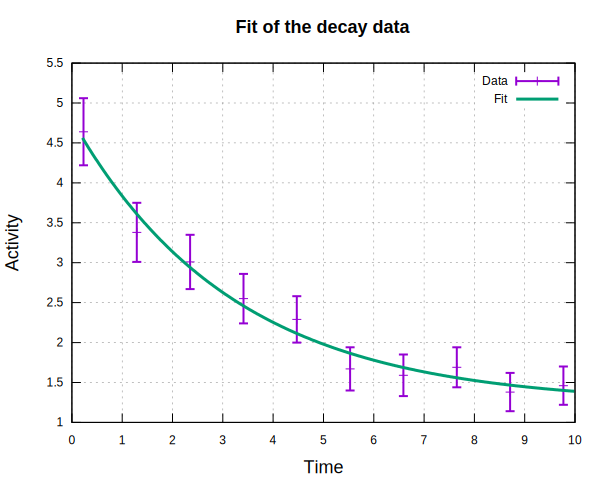
\includegraphics[width=\linewidth]{plot.pdf}
\caption{Homemade figure of the largest Eigenvalues}
\label{fig:1}
\end{centering}
\end{figure}


\end{document}